\documentclass{article}
\usepackage{tikz, comment}
\usepackage{pifont}
\usepackage{fontspec}
\usetikzlibrary{arrows, decorations.markings, decorations.pathreplacing}
\begin{comment}
:Title: Not defined yet
:Slug: No name yet

Description Here.........
\end{comment}
\begin{document}\centering 

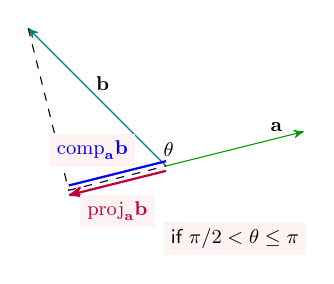
\begin{tikzpicture}[>=latex,xscale=.5*1.75, yscale=.5*1.75][font=\sf\small] 

\draw[green!60!black, ->, >=stealth'] (0, 0) -- ({4*0.5}, {1*0.5})node[black, above, midway, pos=0.8, xshift=0, yshift=0, scale=0.8]{${\bf a}$};

\draw[teal, ->, >=stealth'] (0, 0) -- (-2, 2)node[black, right, midway, pos=0.6, xshift=2, yshift=0, scale=0.8]{${\bf b}$};

\draw[purple, thick, ->, >=stealth', yshift=-2] (0, 0) -- ({-6/17*4}, {-6/17*1})node[below, fill=red!5!white, midway, pos=0.5, xshift=0, yshift=-4, scale=0.8]{$\hbox{\rm proj}_{\bf a} {\bf b}$};

\draw[dashed] (-2, 2) -- ({-6/17*4}, {-6/17*1}) -- (0,0);

\draw[blue, thick, yshift=2] (0, 0) -- ({-6/17*4}, {-6/17*1})node[above, fill=red!5!white, midway, pos=0.7, xshift=-2, yshift=4, scale=0.8]{$\hbox{\rm comp}_{\bf a} {\bf b}$};

\node[xshift=1, yshift=6, scale=0.8] at (0,0) {$\theta$};

\node[black, below, fill=red!5!white, xshift=0, yshift=-20, scale=0.8] at (1,0) {if $\pi/2 < \theta \le \pi$};

\end{tikzpicture}
\end{document}